\documentclass[a4paper,10pt]{article}
\setlength{\parindent}{0cm}
\usepackage{amsmath, amssymb, amsthm, mathtools,pgfplots}
\usepackage{graphicx,caption}
\usepackage{verbatim}
\usepackage{venndiagram}
\usepackage[cm]{fullpage}
\usepackage{fancyhdr}
\usepackage{tikz}
\usepackage{listings}
\usepackage{color,enumerate,framed}
\usepackage{color,hyperref}
\definecolor{darkblue}{rgb}{0.0,0.0,0.5}
\hypersetup{colorlinks,breaklinks,
            linkcolor=darkblue,urlcolor=darkblue,
            anchorcolor=darkblue,citecolor=darkblue}

%\usepackage{tgadventor}
%\usepackage[nohug]{diagrams}
\usepackage[T1]{fontenc}
%\usepackage{helvet}
%\renewcommand{\familydefault}{\sfdefault}
%\usepackage{parskip}
%\usepackage{picins} %for \parpic.
%\newtheorem*{notation}{Notation}
%\newtheorem{example}{Example}[section]
%\newtheorem*{problem}{Problem}
\theoremstyle{definition}
%\newtheorem{theorem}{Theorem}
%\newtheorem*{solution}{Solution}
%\newtheorem*{definition}{Definition}
%\newtheorem{lemma}[theorem]{Lemma}
%\newtheorem{corollary}[theorem]{Corollary}
%\newtheorem{proposition}[theorem]{Proposition}
%\newtheorem*{remark}{Remark}
%\setcounter{section}{1}

\newtheorem{thm}{Theorem}[section]
\newtheorem{lemma}[thm]{Lemma}
\newtheorem{prop}[thm]{Proposition}
\newtheorem{cor}[thm]{Corollary}
\newtheorem{defn}[thm]{Definition}
\newtheorem*{examp}{Example}
\newtheorem{conj}[thm]{Conjecture}
\newtheorem{rmk}[thm]{Remark}
\newtheorem*{nte}{Note}
\newtheorem*{notat}{Notation}

%\diagramstyle[labelstyle=\scriptstyle]

\lstset{frame=tb,
  language=Oz,
  aboveskip=3mm,
  belowskip=3mm,
  showstringspaces=false,
  columns=flexible,
  basicstyle={\small\ttfamily},
  breaklines=true,
  breakatwhitespace=true,
  tabsize=3
}


\pagestyle{fancy}




\fancyhead{}
\renewcommand{\headrulewidth}{0pt}

\lfoot{\color{black!60}{\sffamily Zhangsheng Lai}}
\cfoot{\color{black!60}{\sffamily Last modified: \today}}
\rfoot{\color{black!60}{\sffamily\thepage}}



\begin{document}
\flushright{Zhangsheng Lai\\1002554}
\section*{Statistics: Homework 2}

\begin{enumerate}
\item[6.3] Given $\hat{\theta} = 2\overline{X}_n$ and $X_1, \ldots, X_n \sim \text{Uniform}(0,\theta)$,
\begin{align*}
\text{\sffamily bias}(\hat{\theta}) & =\mathbb{E}(2\overline{X}_n)-\theta\\
& =2n^{-1}\mathbb{E}\left(\sum_{i=1}^{n}{X}_i\right)-\theta\\
& =2n^{-1}\sum_{i=1}^{n}\mathbb{E}\left({X}_i\right)-\theta\\
& =2n^{-1}\frac{n\theta}{2}-\theta=0\\
\text{\sffamily se}(\hat{\theta})^2 & = \mathbb{V}(2\overline{X}_n)\\
& = 4\mathbb{V}(\overline{X}_n)\\
&=4n^{-2}\mathbb{V}\left(\sum_{i=1}^{n}{X}_i\right)\\
&=4n^{-2}\sum_{i=1}^{n}\mathbb{V}\left({X}_i\right)\\
&=4n^{-2}\frac{n\theta^2}{12} = \frac{\theta^2}{3n}\\
\text{\sffamily MSE}(\hat{\theta}) &= \text{bias}(\hat{\theta})^2+\text{se}(\hat{\theta})^2 = \frac{\theta^2}{3n}
\end{align*}
\item[7.2] For $X_1, \ldots, X_n \sim \text{Bernoulli}(p)$ plug-in estimator for $p$ is 
\begin{align*}
\hat{p}=\frac{1}{n}\sum_{i=1}^{n}X_i
\end{align*}
and the estimated standard error is given by
\begin{align*}
\hat{\text{\sffamily se}}_p = \sqrt{\mathbb{V}(\hat{p})} = \sqrt{\frac{\hat{p}(1-\hat{p})}{n} }
\end{align*}
As the $X_i$'s are iid, by Central Limit Theorem, $\hat{p}$ is asymptotically normal with mean $p$ and variance $\hat{\text{\sffamily se}}_p^2$. Thus an approximate $90\%$ confidence interval for $p$ is $(\hat{p}-1.645\text{\sffamily se},\hat{p}+1.645\text{\sffamily se})$.

For $X_1, \ldots, X_n \sim \text{Bernoulli}(p)$ and $Y_1, \ldots, Y_n \sim \text{Bernoulli}(q)$ plug-in estimator for $p-q$ is 
\begin{align*}
\hat{p}-\hat{q}=\frac{1}{n}\sum_{i=1}^{n}X_i - \frac{1}{m}\sum_{i=1}^{m}Y_i
\end{align*}
with estimated standard error 
\begin{align*}
\hat{\text{\sffamily se}}_{p-q} = \sqrt{\mathbb{V}(\hat{p}-\hat{q})} = \sqrt{\mathbb{V}(\hat{p})+\mathbb{V}(\hat{q})}= \sqrt{\frac{\hat{p}(1-\hat{p})}{n}+\frac{\hat{q}(1-\hat{q})}{m} }
\end{align*}
Since the $Y_i$'s are iid, by Central Limit Theorem $\hat{q}$ is asymptotically normal with mean $q$ and variance $\hat{\text{\sffamily se}}_q^2$. The difference of two asymptotically normal random variables is asymptotically normal, thus $\hat{p-q}$ is asymptotically normal with mean $p-q$ and variance $\text{\sffamily se}_{p-q}^2$. An approximate $90\%$ confidence interval is 
\begin{align*}
%\text{\sffamily se}_{p-q}=
(\hat{p}-\hat{q}-1.645\text{\sffamily se}_{p-q},\hat{p}-\hat{q}+1.645\text{\sffamily se}_{p-q})
\end{align*}
\item[7.9] An estimate for $p_1-p_2$ is $0.9-0.85=0.05$ with standard error 
\begin{align*}
\sqrt{\frac{0.9(1-0.9)}{100}+\frac{0.85(1-0.85)}{100}}= 0.0466368953
\end{align*}
with $80\%$ and $90\%$ confidence intervals given by
\begin{align*}
80\%:\quad(\hat{p}-\hat{q}-1.282\text{\sffamily se}_{p-q},\hat{p}-\hat{q}+1.282\text{\sffamily se}_{p-q})&=(-0.0097885,0.1097885)\\
90\%:\quad(\hat{p}-\hat{q}-1.96\text{\sffamily se}_{p-q},\hat{p}-\hat{q}+1.96\text{\sffamily se}_{p-q})&=(-0.041408315,0.141408315)
\end{align*} 

\item[8.7]
\begin{enumerate}[(a)]
\item 
\begin{align*}
\mathbb{P}(\hat{\theta}\leq k) &= \mathbb{P}(\max\{X_1,\ldots,X_n\}\leq k)\\
&= \prod_{i=1}^{n}\mathbb{P}(X_i\leq k)\\
&=\left(\frac{k}{\theta}\right)^n
\end{align*}
\begin{figure}[h]
\centering
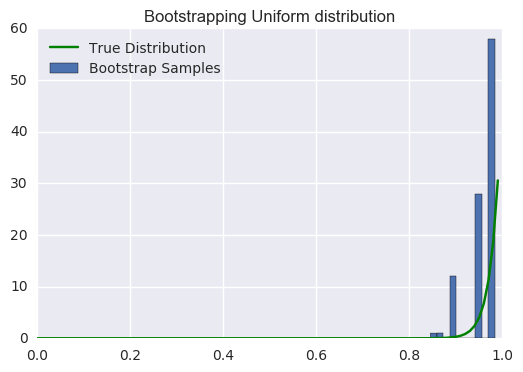
\includegraphics[scale=1]{bootstrap.png}
\caption{Comparison of the true distribution $\hat{\theta}$ to histrograms from bootstrap}
\end{figure}
\item Let $\hat{\theta} = X_{max} = \max\{X_1, \ldots, X_n\}$. Then
\begin{align*}
\mathbb{P}(\hat{\theta}^\ast = \hat{\theta})&=1-\mathbb{P}(\hat{\theta}^\ast \neq \hat{\theta})\\
&=1 - \left(1-\frac{1}{n}\right)^n
\end{align*}
The second equality holds as $\mathbb{P}(\hat{\theta}^\ast \neq \hat{\theta})$ denotes the probability that any random sampling with replacement of the $n$ samples drawn has probability of $1-1/n$ not being $x_{max}$ (which is fixed since a random sample of $n$ has been drawn). As each sampling process is iid due to replacement, probability of them all not being $x_{max}$ is $(1-1/n)^n$. Thus we have $\mathbb{P}(\hat{\theta}^\ast = \hat{\theta}) \to 0$ as $n \to \infty$ and $\mathbb{P}(\hat{\theta}^\ast = \hat{\theta}) = .632$ for $n=50$.
\end{enumerate}
\item[9.2]
\begin{enumerate}[(a)]
\item For $X_1,\ldots, X_n \sim \text{Uniform}(a,b)$
\begin{align*}
\hat{\mu}=\overline{X}_n=\frac{1}{n}\sum_{i=1}^{n}X_i&=\frac{\hat{b}+\hat{a}}{2}\\
\hat{\sigma}^2=\frac{1}{n}\sum_{i=1}^{n}(\overline{X}_n-X_i)^2&=\frac{(\hat{b}-\hat{a})^2}{12}
\end{align*}
thus
\begin{align*}
(\hat{b}-\hat{a})+(\hat{b}+\hat{a}) &= +\sqrt{12\hat{\sigma}^2}+2\hat{\mu}\\
\hat{b} &= \frac{1}{2}\left(\sqrt{12\hat{\sigma}^2}+2\hat{\mu}\right)\\
\hat{a} &=2\hat{\mu}-\hat{b }
\end{align*}
the positive root is taken as $b-a>0$.
\item Let $X_1,\ldots, X_n \sim \text{Uniform}(a,b)$, with $X_{max}=\max \{X_1,\ldots, X_n\}$. If $b < X_{max}$, then $f(X_j;a,b)=0$ for some $j$. Thus if $b \geq X_{max}$, then $f(X_i;a,b)=1/b-a$ for all $i$. In a similar fashion, letting $X_{min} = \{X_1,\ldots, X_n\}$, if $X_{min}<a$ we also have $f(X_j;a,b)=0$ for some $j$ and $f(X_i;a,b)=1/b-a$ for all $i$ if $X_{min} \geq a$. Therefore,
\begin{align*}
\mathcal{L}_n(a,b):=\begin{cases}
0, & X_{min} < a \text{ or }X_{max} >  b \\
\left(\frac{1}{b-a}\right)^n, & \text{ otherwise }%X_{max} \leq b \text{ and } X_{min} \geq a
\end{cases}
\end{align*}
$\mathcal{L}(a,b)$ strictly decreasing over $(-\infty,X_{min}]$ and $[X_{max},\infty)$, thus the maximum likelihood estimators $\hat{a}=X_{min}$ and $\hat{b}=X_{max}$.

\item Let $\tau = \int x \,dF(x)$ be given, then from (b) we know that {\sffamily MLE}'s $\hat{a}$ and $\hat{b}$ are given by $X_{min}$ and $X_{max}$ respectively. Then the {\sffamily MLE} of $\tau$ follows from {\sffamily MLE}'s $\hat{a}$ and $\hat{b}$. Thus {\sffamily MLE} of $\tau$ is $(X_{min} + X_{max})/2$. 
\item
\end{enumerate}
\item[9.6] 

\end{enumerate}

\end{document}